\documentclass[11pt,reqno]{amsart}
\usepackage[a4paper,margin=28mm]{geometry}
\usepackage[T1]{fontenc}
\usepackage{lmodern}
\usepackage{amsmath,amssymb,mathtools}
\usepackage[expansion=false]{microtype}
\usepackage{xcolor,booktabs,array,enumitem,needspace}
\usepackage{tikz}
\usetikzlibrary{arrows.meta,positioning,calc}
\definecolor{linkteal}{RGB}{0,85,91}
\usepackage[colorlinks=true,linkcolor=linkteal,citecolor=linkteal,urlcolor=linkteal,
 pdfauthor={Harjas Sandhu},
 pdftitle={Quantum Memory from Rare Thermal Boundaries},
 pdfsubject={Exact-dynamics storage criteria and the role of thermal preparation}]{hyperref}
\usepackage[nameinlink,noabbrev]{cleveref}
\numberwithin{equation}{section}
\newtheorem{theorem}{Theorem}[section]
\newtheorem{proposition}[theorem]{Proposition}
\newtheorem{corollary}[theorem]{Corollary}
\newtheorem{lemma}[theorem]{Lemma}
\theoremstyle{definition}
\newtheorem{definition}[theorem]{Definition}
\newtheorem{example}[theorem]{Example}
\newtheorem{assumption}[theorem]{Assumption}
\theoremstyle{remark}
\newtheorem{remark}[theorem]{Remark}
\newcommand{\Tr}{\operatorname{Tr}}
\newcommand{\id}{\operatorname{id}}
\newcommand{\Ad}{\operatorname{Ad}}
\newcommand{\supp}{\operatorname{supp}}
\newcommand{\Rea}{\operatorname{Re}}
\newcommand{\ran}{\operatorname{ran}}
\newcommand{\Bcal}{\mathcal B}
\newcommand{\Hcal}{\mathcal H}
\newcommand{\Ncal}{\mathcal N}
\newcommand{\Ecal}{\mathcal E}
\newcommand{\Wcal}{\mathcal W}
\newcommand{\Ccal}{\mathcal C}
\newcommand{\Dcal}{\mathcal D}
\newcommand{\dd}{\mathrm d}
\newcommand{\Fe}{F_{\mathrm e}}
\newcommand{\diam}{d_\diamond}
\newcommand{\one}{\mathbf 1}
\newcommand{\pa}{\mathfrak a}
\DeclarePairedDelimiter{\norm}{\lVert}{\rVert}
\DeclarePairedDelimiter{\abs}{\lvert}{\rvert}
\DeclareMathOperator{\dist}{dist}
\DeclareMathOperator{\Dom}{Dom}
\setlist[enumerate]{leftmargin=*,itemsep=3pt,topsep=5pt}
\setlist[itemize]{leftmargin=*,itemsep=3pt,topsep=5pt}
\allowdisplaybreaks[2]
\setlength{\emergencystretch}{1.5em}
\title[Quantum memory from rare thermal boundaries]{Quantum Memory from Rare Thermal Boundaries}
\author{Harjas Sandhu}
\address{The University of Queensland}
\email{harjas.sandhu@student.uq.edu.au}
\date{6 November 2026}
\subjclass[2020]{81P45, 82B10, 81P48, 46L55}
\keywords{quantum memory, Gibbs state, exact Hamiltonian dynamics, relative entropy, quantum channels, noiseless subsystems}
\begin{document}
\begin{abstract}
A logical observable can change slowly because its commutator with the
Hamiltonian is supported on a thermally rare subspace. Turning this observation
into a memory theorem requires control of the state after an unknown input has
been written. We give two complete criteria for that step under the exact joint
system--bath dynamics. If all three logical Pauli commutators are supported on
a common projection of Gibbs probability \(p\), with summed norm bound
\(\pa\), ideal subsystem replacement gives deterministic half-diamond error
at most \(\pa p|t|F(\beta\pa/4)\), where
\(F(K)=\inf_{\lambda>0}(K+e^\lambda-1)/\lambda\).
A Pauli-randomized protocol instead has error at most
\(\pa p(2|t|+\beta)/4\).
The proofs use rare-event relative entropy and a Bell-projection identity,
respectively. The latter identity also gives a dimension-independent
correlation criterion for arbitrary correlated resources and arbitrary joint
quantum channels, including an algebraic infinite-bath formulation.
We identify precise sufficient conditions for imperfect writing and prove that
global domination by a thermal encoder can fail exponentially even for harmless
independent gauge faults. All storage statements assume a specified accessible
logical algebra and a fixed joint resource; preparation cost and a generic
noisy-writing threshold are not supplied. The results are abstract criteria,
rather than a new three-dimensional memory construction.
\end{abstract}
\maketitle
\setcounter{tocdepth}{1}
\tableofcontents
\clearpage
\section{Introduction}\label{sec:introduction}

A passive quantum memory must preserve an unknown state, including its
entanglement with a reference, without active correction. Thermal equilibrium
can help when logical errors must pass through configurations of small Gibbs
weight. But an unknown input is not an equilibrium state. A correlation
estimate becomes a memory theorem only after writing, holding and reading
operations have been specified.

This paper studies that passage. Its basic hypothesis is an exact operator
identity. The accessible physical system contains a full logical qubit algebra,
and each logical Pauli commutator with the \emph{actual joint Hamiltonian}
is supported on a common projection \(P\). We call \(P\) a thermal boundary:
outside its range the instantaneous logical derivative vanishes. This name
does not assert that \(P\) is a geometric surface, an energy eigenspace or an
invariant subspace. In particular, \(P\) need not commute with the Hamiltonian
or its Gibbs state.

The main theorem turns the equilibrium probability
\[
                  p=\Tr(\omega P),\qquad
                  \omega=\frac{e^{-\beta H}}{\Tr e^{-\beta H}},
\]
into a bound on the entire memory channel. An ideal logical swap retains the
joint marginal of the other physical variables and bath.
Its relative-entropy cost, on a maximally mixed input, is \(O(p)\).
A binary entropy estimate keeps the boundary probability \(O(p)\) at all
times, and integration gives logical error \(O(p|t|)\).
A second proof uses thermal correlations and a classical Pauli frame.
Both concern exact joint dynamics.

\subsection{Relation to established approaches}

The correlation-and-fidelity framework is established.
Alicki and Fannes \cite{AF09}, Sections~2--4, treat encoded matrix algebras,
correlated invariant resources and CP dynamics, including logical replacement
with a fixed syndrome marginal. The replacement used here belongs to
that framework.

Theorem~1 of Chesi, Loss, Bravyi and Terhal \cite{CLBT10} already bounds
memory error by \(t\) times a bad-syndrome Gibbs probability for
Gibbs-stationary Markovian dynamics of stabilizer and subsystem codes.
Inverse-rarity storage is therefore a known mechanism. Our hypotheses
instead concern total-Hamiltonian commutators and the interacting
system--bath Gibbs state.

Balasubramanian, Davydova and Lin \cite{BDL26}, Theorems~3.16 and 5.13
and Corollary~5.14, give a three-dimensional local stabilizer construction
with long thermal storage under their stationary dynamics.
Bergamaschi, Gheissari and Liu \cite{BGL25}, Theorem~1.7 and formal
Theorem~7.8, address thermalization within a logical sector under
additional code and sampler hypotheses.

Rakovszky, Placke, Breuckmann and Khemani \cite{RPBK26}, Theorem~2 and
Supplement~II, control mixing through quantum bottlenecks, including
off-diagonal contributions. Slow mixing alone does not preserve a coherent
qubit. Ma, Khemani and Sang \cite{MKS26}, Theorems~1--3, relate phase
transport and self-correction under stronger clustering and local
stationary-dynamics assumptions.

\subsection{Contribution and organization}

\Cref{thm:main} gives the two exact-dynamics storage criteria.
\Cref{thm:bell} separates an arbitrary-resource channel statement from
its thermal input; \cref{sec:writing} treats imperfect writing.
The appendices give an infinite-bath interface, counterexamples and a
separate collective-symmetry application.
Data processing, Bell projection, channel twirling and noiseless
subsystems are established machinery; no firstness is claimed for them.
The contribution is the stated criteria and their proofs, with their
dependencies explicit. A new local construction, efficient resource
preparation and a noisy-writing threshold are separate tasks.

\clearpage
\section{The mechanism in one page}\label{sec:overview}

Think of the memory as a logical qubit \(L\), accessible auxiliary variables
\(A\), and a bath \(B\) that cannot be controlled. The auxiliary variables and
bath may be correlated with each other and with the old logical qubit.
An external input is swapped into \(L\); the old logical qubit is discarded.
The state left behind on \(G=A B\) is its original marginal \(\omega_G\).
This is a legitimate input-independent quantum channel.

\begin{center}
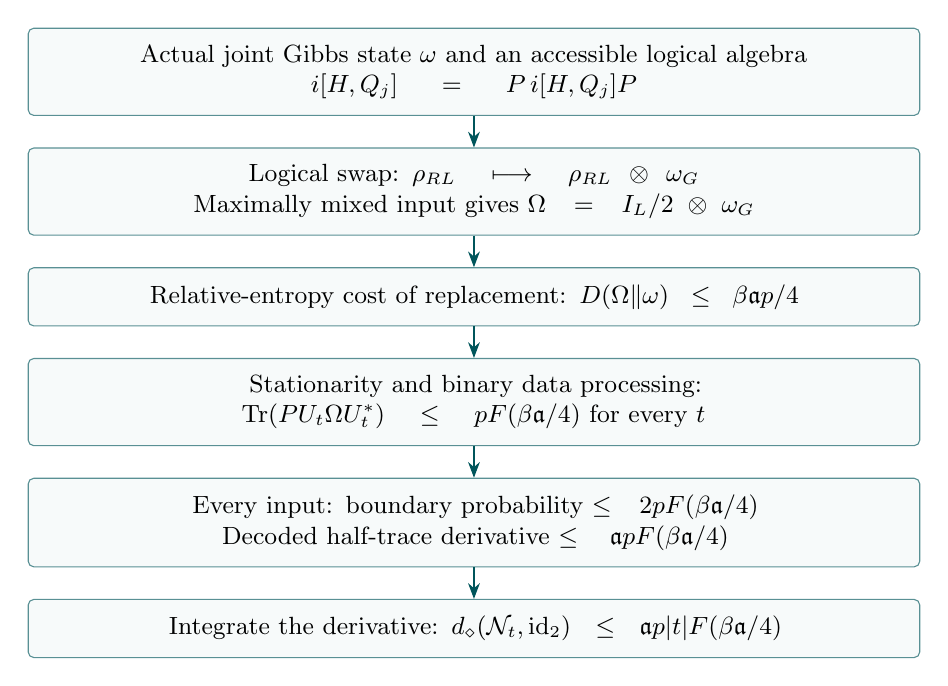
\begin{tikzpicture}[
 box/.style={draw=linkteal!65,fill=linkteal!3,rounded corners=2pt,
 text width=10.9cm,align=center,inner sep=6pt,font=\small},
 >={Stealth[length=2mm]},node distance=4mm]
\node[box] (resource) {Actual joint Gibbs state \(\omega\) and an accessible
 logical algebra\\ \(i[H,Q_j]=P\,i[H,Q_j]P\)};
\node[box,below=of resource] (write) {Logical swap:
 \(\rho_{RL}\longmapsto\rho_{RL}\otimes\omega_G\)\\
 Maximally mixed input gives \(\Omega=I_L/2\otimes\omega_G\)};
\node[box,below=of write] (entropy) {Relative-entropy cost of replacement:
 \(D(\Omega\Vert\omega)\le \beta\pa p/4\)};
\node[box,below=of entropy] (probability) {Stationarity and binary data processing:
 \(\Tr(PU_t\Omega U_t^*)\le pF(\beta\pa/4)\) for every \(t\)};
\node[box,below=of probability] (drift) {Every input: boundary probability
 \(\le 2pF(\beta\pa/4)\)\\
 Decoded half-trace derivative \(\le\pa pF(\beta\pa/4)\)};
\node[box,below=of drift] (error) {Integrate the derivative:
 \(\diam(\Ncal_t,\id_2)\le\pa p|t|F(\beta\pa/4)\)};
\foreach \a/\b in {resource/write,write/entropy,entropy/probability,
probability/drift,drift/error}
\draw[->,linkteal] (\a)--(\b);
\end{tikzpicture}
\end{center}

Here \(\pa\) is the sum of the three commutator norm bounds.
The crucial operation is the fourth line. A general trace-distance estimate
from relative entropy would introduce a square root of \(p\). Instead,
we ask only about the particular event \(P\); its binary relative entropy
controls a change from probability \(p\) to a constant multiple of \(p\).

There is a second route. A Bell-state test turns a complete set of logical
correlation estimates into entanglement fidelity. A random Pauli before
writing, followed by its inverse after reading, converts that fidelity
into an exact half-diamond error for the averaged channel. Thermal
weighted correlations then give the bound
\(\pa p(2|t|+\beta)/4\).
This protocol retains two classical frame bits reliably during storage.
Neither route prepares \(\omega\) or makes a nonlocal logical swap inexpensive.

\clearpage
\section{Setup and the main storage theorem}\label{sec:results}

\subsection{Access, resource and error criterion}

All Hilbert spaces in the main theorem are finite-dimensional. Let the
accessible physical system have a specified subsystem identification
\[
             \Hcal_S\simeq\Hcal_L\otimes\Hcal_A,
             \qquad \Hcal_L=\mathbb C^2,
             \qquad \Hcal_G=\Hcal_A\otimes\Hcal_B.
\]
The identification must be implementable using the system alone. It need
not be geometrically local or efficient. Let \(H=H^*\) act on \(L G\),
and let \(Q_x,Q_y,Q_z\) be the ordinary Pauli matrices on \(L\), extended
by the identity. They satisfy the Pauli algebra on the \emph{whole}
physical Hilbert space, rather than only on a selected low-energy sector.
We use units \(\hbar=k_{\mathrm B}=1\).

An external logical input, independent of a fixed resource state \(\omega\),
is swapped into \(L\). Tracing the old logical register gives
\begin{equation}\label{eq:encoder}
 \Ecal(\rho)=\rho\otimes\omega_G,\qquad
 \omega_G=\Tr_L\omega .
\end{equation}
This identity holds also for inputs entangled with an arbitrary reference.
No bath operation or conditional re-equilibration is involved.
Holding and reading give the channel
\begin{equation}\label{eq:memory}
 \Ncal_t(\rho)=\Tr_G\!\left[U_t(\rho\otimes\omega_G)U_t^*\right],
 \qquad U_t=e^{-itH}.
\end{equation}
Reading means recovering the specified \(L\) factor and discarding \(A\);
the bath is inaccessible throughout.

For channels with the same input and output, write
\[
 \diam(\Ncal,\mathcal M)=\tfrac12\norm{\Ncal-\mathcal M}_\diamond.
\]
Equivalently, this is the supremum of half the output trace norm over
reference-entangled inputs. This operational error lies in \([0,1]\).
In particular \(\Ncal_0=\id_2\).

The randomized protocol chooses \(Q\) uniformly from
\(\{I,Q_x,Q_y,Q_z\}\), applies it to the external input before writing,
and applies \(Q^*\) to the decoded output. Its channel is
\begin{equation}\label{eq:twirl}
 \widetilde{\Ncal}_t=
 \frac14\sum_Q\Ad(Q^*)\circ\Ncal_t\circ\Ad(Q),
 \qquad \Ad(V)(\rho)=V\rho V^*.
\end{equation}
The resource and holding dynamics are independent of this choice.
The guarantee for \(\widetilde{\Ncal}_t\) averages over the classical choice;
it is not a guarantee for each fixed seed.

\subsection{An exact rare-boundary hypothesis}

Suppose
\begin{equation}\label{eq:gibbs}
          \omega=Z^{-1}e^{-\beta H},
          \qquad Z=\Tr e^{-\beta H},\quad 0\le\beta<\infty.
\end{equation}
Let \(P\) be an orthogonal projection and suppose, for \(j=x,y,z\),
\begin{equation}\label{eq:support}
 [P,Q_j]=0,\qquad
 A_j:=i[H,Q_j]=P A_jP,\qquad
 \norm{A_j}\le a_j .
\end{equation}
Define
\begin{equation}\label{eq:parameters}
           p=\Tr(\omega P),\qquad \pa=a_x+a_y+a_z.
\end{equation}
The two-sided support identity in \eqref{eq:support} is stronger than
a small Gibbs expectation of \(A_j^2\). It says that the logical
velocity vanishes exactly unless the state meets the boundary.
We assume neither \([P,H]=0\) nor \([P,\omega]=0\).

For \(K\ge0\) set
\begin{equation}\label{eq:F}
 F(K)=\inf_{\lambda>0}\frac{K+e^\lambda-1}{\lambda}.
\end{equation}
Thus \(F(0)=1\), and the choice \(\lambda=1\) gives
\(F(K)\le K+e-1\).

\Needspace{17\baselineskip}
\begin{theorem}[Storage from a thermal boundary]\label{thm:main}
Under \eqref{eq:gibbs}--\eqref{eq:parameters}, with the ideal access protocol
\eqref{eq:encoder}--\eqref{eq:memory}, for every real \(t\),
\begin{align}
 \diam(\Ncal_t,\id_2)
 &\le \min\{1,\pa p|t|F(\beta\pa/4)\},                 \label{eq:deterministic}\\
 \diam(\widetilde{\Ncal}_t,\id_2)
 &\le \min\{1,\tfrac14\pa p(2|t|+\beta)\}.            \label{eq:randomized}
\end{align}
The randomized channel also obeys the bound in \eqref{eq:deterministic} and
\begin{equation}\label{eq:quadratic-main}
 \diam(\widetilde{\Ncal}_t,\id_2)
 \le \min\{1,\tfrac14pt^2(a_x^2+a_y^2+a_z^2)\}.
\end{equation}
The minimum of these bounds may be used. In particular its error vanishes
at \(t=0\), although the right side of \eqref{eq:randomized} alone
has a nonzero constant term when \(\beta\pa p>0\).
\end{theorem}

The proof of \eqref{eq:deterministic} is in \cref{sec:entropy}.
The general channel theorem in \cref{sec:channel} and the thermal estimate
in \cref{sec:thermal} prove the remaining bounds. None of the constants
contains the bath dimension. An estimate uniform in bath volume still
requires \(p\) and \(a_j\) themselves to be uniform in that volume.

\begin{corollary}[Conditional stretched-exponential storage]\label{cor:asymptotic}
Suppose a sequence of models satisfies the theorem, and separately
established estimates give
\[
 p_n\le Cn^r e^{-c n^\eta},\qquad
 \pa_n\le C'n^s,\qquad 0\le\beta_n\le\beta_*<\infty,
\]
where \(c,\eta,C,C'>0\), \(r,s\ge0\) and all constants are independent
of \(n\). For every \(0<\varepsilon<c\), both the deterministic and
randomized errors tend uniformly to zero on
\[
                  |t|\le e^{(c-\varepsilon)n^\eta}.
\]
\end{corollary}
\begin{proof}
The estimate \(F(K)\le K+e-1\) bounds the deterministic error by a polynomial
in \(n\) times \(e^{-\varepsilon n^\eta}\). The same is true of
\eqref{eq:randomized}; twirling is also contractive in diamond norm.
\end{proof}

This is a consequence of a supplied equilibrium estimate, not a method for
proving it. Geometry, disorder strength, interaction range, energy scales
and a temperature interval enter through that separate task. In
particular, bath-only terms vanish from the logical commutators but can
still change \(p\).

\begin{example}[A two-qubit boundary that can be computed exactly]
\label{ex:two-qubit}
Take one logical and one gauge qubit, \(n=|1\rangle\langle1|_G\), and
\[
              H=I_L\otimes\Delta n+gQ_z\otimes n.
\]
Here \(P=I_L\otimes n\), \(a_x=a_y=2|g|\), and \(a_z=0\).
The actual Gibbs probability is
\[
       p=\frac{e^{-\beta\Delta}\cosh(\beta g)}
                  {1+e^{-\beta\Delta}\cosh(\beta g)}.
\]
After replacement the gauge qubit has this same population, so
\[
 \Ncal_t=(1-p)\id_2+p\Ad(e^{-igtQ_z}).
\]
Its half-diamond error is \(p|\sin(gt)|\). Indeed, the two eigenvalues
of \(e^{-igtQ_z}\) give the unitary-channel distance
\(|\sin(gt)|\), attained on an equatorial qubit; the mixture scales
the channel difference by \(p\). Pauli randomization removes the
coherent \(Z\) rotation term and gives
\(\widetilde{\Ncal}_t=(1-p\sin^2(gt))\id_2+
p\sin^2(gt)\Ad(Q_z)\), with error \(p\sin^2(gt)\).
The exact error is at most \(p\) for all times. Thus the
inverse-\(p\) storage interval in the theorem is a sufficient estimate,
not an asserted optimal lifetime for every model.
\end{example}

\section{Relative entropy keeps a rare boundary rare}\label{sec:entropy}

The deterministic proof has two ingredients. First, a writer whose average
output has relative-entropy cost \(O(p)\) cannot increase the probability of
a Gibbs event of weight \(p\) by more than a constant factor. Second, the
support identities turn that probability directly into a bound on the
logical channel derivative. We prove these statements before checking the
thermal replacement writer.

For states \(\sigma,\omega\), with \(\omega\) faithful, use natural logarithms
and write
\[
 D(\sigma\Vert\omega)=\Tr\sigma(\log\sigma-\log\omega).
\]
For \(q,p\in(0,1)\), write
\[
 d(q\Vert p)=q\log(q/p)+(1-q)\log((1-q)/(1-p))
\]
for binary relative entropy, with its continuous endpoint conventions.
We use data processing under completely positive trace-preserving maps.
Theorem~1 of M\"uller-Hermes and Reeb \cite{MHR17} implies the version needed
here: relative entropy decreases under a positive trace-preserving map
between finite-dimensional trace-class spaces. Our maps are the binary
measurement and the partial trace of a finite classical flag, so they
satisfy its hypotheses. The older completely positive result is due to
Lindblad \cite{Lindblad75}.

\begin{lemma}[A binary rare-event bound]\label{lem:binary}
Let \(P\) be a projection, \(p=\Tr(\omega P)\), and \(q=\Tr(\sigma P)\).
If \(D(\sigma\Vert\omega)\le Kp\), then
\begin{equation}\label{eq:binary}
                         q\le pF(K).
\end{equation}
\end{lemma}
\begin{proof}
Suppose first \(0<p<1\). Measuring \(\{P,I-P\}\) gives
\(d(q\Vert p)\le Kp\). For \(\lambda>0\), set
\[
 p_\lambda=\frac{pe^\lambda}{1-p+pe^\lambda}.
\]
Expanding \(d(q\Vert p_\lambda)\ge0\) yields
\[
 \lambda q
 \le d(q\Vert p)+\log(1-p+pe^\lambda)
 \le p(K+e^\lambda-1),
\]
where \(\log(1+x)\le x\) was used in the last step.
Take the infimum over \(\lambda\).
For \(p=0\), faithfulness of \(\omega\) implies \(P=0\); for \(p=1\),
\(q\le1\le F(K)\).
\end{proof}

The lemma asks only about one rare event. For example,
\(D(\sigma\Vert\omega)\le10p\) gives
\(q\le(10+e-1)p\), however small \(p\) is. A general trace-distance
estimate based on Pinsker's inequality would instead allow an additive
error of order \(\sqrt p\). That weaker estimate loses information
relevant to the storage timescale.

\begin{lemma}[Logical drift with an arbitrary reference]\label{lem:drift}
Suppose \eqref{eq:support} holds and \(\rho_{LGR}(t)\) follows the joint
Hamiltonian evolution, with the identity on the reference \(R\).
Put \(q_\rho(t)=\Tr(P\rho_{LG}(t))\) and
\(\rho_{LR}(t)=\Tr_G\rho_{LGR}(t)\). Then
\begin{equation}\label{eq:drift}
          \tfrac12\norm{\dot\rho_{LR}(t)}_1
                    \le \tfrac12\pa q_\rho(t).
\end{equation}
\end{lemma}
\begin{proof}
Expand the logical qubit in its Pauli basis:
\[
 \rho_{LR}(t)=\tfrac12 I_L\otimes\rho_R+
                 \tfrac12\sum_{j=x,y,z}Q_j\otimes C_j(t).
\]
The reference marginal is constant. Differentiating and using the
Hamiltonian equation gives
\[
 \dot C_j(t)=
   \Tr_{LG}\big[(A_j\otimes I_R)\rho_{LGR}(t)\big].
\]
This is Hermitian. For any Hermitian reference contraction \(B\),
the support and norm hypotheses imply the operator inequalities
\[
 -a_j P\otimes I_R\le A_j\otimes B\le a_j P\otimes I_R.
\]
Consequently \(|\Tr B\dot C_j(t)|\le a_jq_\rho(t)\).
Trace-norm duality gives \(\norm{\dot C_j(t)}_1\le a_jq_\rho(t)\).
Since \(\norm{Q_j}_1=2\), the Pauli expansion proves
\eqref{eq:drift}. No bound depends on the reference dimension.
\end{proof}

\begin{theorem}[An entropy condition for a writer]\label{thm:entropy-writer}
Let \(H\) act on a logical qubit and \(G\), and let \(\omega\) be a faithful
state invariant under \(U_t=e^{-itH}\). Assume \eqref{eq:support}.
Let \(\Gamma:\Bcal(L)_*\to\Bcal(LG)_*\) be a CPTP writing channel,
and put \(\sigma=\Gamma(I_L/2)\), \(p=\Tr(\omega P)\).
Suppose
\[
 D(\sigma\Vert\omega)\le Kp,\qquad
 \diam(\Tr_G\Gamma,\id_2)\le\varepsilon_0.
\]
Then, for all real \(t\),
\begin{equation}\label{eq:entropy-writer}
 \diam(\Tr_G\Ad(U_t)\Gamma,\id_2)
       \le\min\{1,\varepsilon_0+\pa p|t|F(K)\}.
\end{equation}
\end{theorem}
\begin{proof}
Unitary invariance and stationarity give
\(D(U_t\sigma U_t^*\Vert\omega)=D(\sigma\Vert\omega)\).
By \cref{lem:binary},
\[
             \Tr(PU_t\sigma U_t^*)\le pF(K)
                       \quad\text{for every }t .
\]
For any input marginal \(\rho_L\le I_L\), positivity of \(\Gamma\) gives
\(\Gamma(\rho_L)\le\Gamma(I_L)=2\sigma\).
Thus every input, including one correlated with a reference, has
physical boundary probability at most \(2pF(K)\).
\Cref{lem:drift} bounds the half trace norm of its decoded derivative by
\(\pa pF(K)\). Integrate from \(0\) to \(t\), include the initial
channel error \(\varepsilon_0\), and take the reference supremum.
\end{proof}

This theorem concerns the actual joint output of the writer. It is a
sufficient condition, not a necessary condition for useful storage.
When \(p\) is exponentially small, the requirement \(D(\sigma\Vert\omega)=O(p)\)
is strong. It is not a constant-noise writing threshold.

\subsection{The Gibbs replacement calculation}

\begin{lemma}[Entropy cost of logical replacement]\label{lem:reset-entropy}
Under \eqref{eq:gibbs}--\eqref{eq:parameters},
\[
 \Omega:=I_L/2\otimes\omega_G
       =\tfrac14\sum_{Q\in\{I,Q_x,Q_y,Q_z\}}Q\omega Q,
 \qquad
 D(\Omega\Vert\omega)\le\tfrac14\beta\pa p.
\]
\end{lemma}
\begin{proof}
The first equality is the Pauli depolarization identity on \(L\);
it can also be checked by expanding \(\omega\) in the Pauli basis.
The Gibbs formula and unitary invariance of entropy give
\[
 D(Q_j\omega Q_j\Vert\omega)
       =\beta\Tr\omega(Q_jHQ_j-H).
\]
Now \(Q_jHQ_j-H=-iQ_jA_j\). This operator is Hermitian, has norm at
most \(a_j\), and is supported on \(P\) on both sides because
\([P,Q_j]=0\). Therefore
\begin{equation}\label{eq:conjugate-entropy}
       D(Q_j\omega Q_j\Vert\omega)\le\beta a_j p.
\end{equation}
To average these inequalities without an additional assumption, attach
a classical flag to the four states \(Q\omega Q\), with weights \(1/4\),
and compare with the flagged state having \(\omega\) in every block.
Their relative entropy is the average of the four relative entropies.
Tracing the flag and using data processing proves the claimed inequality.
\end{proof}

\begin{proof}[Proof of \eqref{eq:deterministic} in \cref{thm:main}]
Apply \cref{thm:entropy-writer} with
\(\Gamma=\Ecal\), \(\sigma=\Omega\), \(K=\beta\pa/4\),
and \(\varepsilon_0=0\), using \cref{lem:reset-entropy}.
\end{proof}

The same proof explains the role of the actual interacting Gibbs state.
Replacing \(\omega\) by an uncoupled reference state would generally destroy
both stationarity and \eqref{eq:conjugate-entropy}. Small interaction norm
alone does not justify that substitution; see \cref{ex:gibbs-comparison}.

\section{From correlations to a complete memory channel}\label{sec:channel}

The second route begins with a statement that needs no thermal assumption.
The input is written into a logical factor of an arbitrary fixed resource.
A complete operator basis tests how much that factor changes during a
joint channel. A Bell projection converts these tests into a memory
fidelity bound without assigning an input-dependent state to the bath.

\subsection{General logical dimension}

Let \(L=\mathbb C^d\) and \(G\) be finite-dimensional, let \(\omega\) be
any state on \(LG\), and let \(\Lambda\) be any CPTP map on \(LG\).
There is no rank, invariance or Gibbs assumption on \(\omega\).
Define
\[
 \Ncal(\rho)=\Tr_G\Lambda(\rho\otimes\omega_G).
\]
Choose the discrete Weyl operators \(W_a\), \(a\in\mathbb Z_d^2\),
with \(W_0=I\), \(W_a^*W_a=I\), and
\(\Tr(W_a^*W_b)=d\delta_{ab}\). Explicitly they are the products of
the cyclic shift and the diagonal phase with entries
\(1,e^{2\pi i/d},\ldots,e^{2\pi i(d-1)/d}\).
They form a projective group.

Let \(\Phi=|\phi\rangle\langle\phi|\), where
\(|\phi\rangle=d^{-1/2}\sum_{j=1}^d|j\rangle_R|j\rangle_L\).
The entanglement fidelity is
\[
             \Fe(\Ncal)=\Tr\Phi\,(\id_R\otimes\Ncal)(\Phi).
\]
Write \(\Lambda^*\) for the unital Heisenberg adjoint, and set
\begin{equation}\label{eq:general-errors}
 e_a=2-2\Rea\Tr\omega W_a^*\Lambda^*(W_a),
 \qquad \bar e=d^{-2}\sum_a e_a.
\end{equation}

\begin{theorem}[Bell--Weyl channel criterion]\label{thm:bell}
With the preceding definitions, each \(e_a\ge0\), and the complete-channel
Weyl randomization
\[
 \widetilde{\Ncal}
   =d^{-2}\sum_a\Ad(W_a^*)\circ\Ncal\circ\Ad(W_a)
\]
satisfies
\begin{equation}\label{eq:bell-result}
 \diam(\widetilde{\Ncal},\id_d)
             =1-\Fe(\Ncal)\le\min\{1,\bar e\}.
\end{equation}
The resource and joint channel must be fixed independently of the
randomization seed.
\end{theorem}

This is a complete input--output guarantee, including arbitrary references.
Its bound has no dimension factor, even if \(d\) grows. The protocol still
requires access to the logical algebra and a reliable classical frame with
\(d^2\) possible values. For \(d=2^k\), one may use the tensor-Pauli group
and store exactly \(2k\) frame bits.

\subsection{Why Bell compression resolves the resource correlation}

Before proving the theorem, consider what a Bell test does to the resource.
Place an independent maximally mixed reference beside \(\omega\):
\[
             \Xi=I_R/d\otimes\omega,\qquad
             \Pi=\Phi_{RL}\otimes I_G.
\]
Projecting \(RL\) onto its Bell state removes its old logical correlations
and leaves the same marginal \(\omega_G\). The precise normalization is
\begin{equation}\label{eq:compression}
                d^2\Pi\Xi\Pi=\Phi_{RL}\otimes\omega_G.
\end{equation}
To verify it, write
\(\omega=\sum_{i,j}|i\rangle\langle j|_L\otimes\omega_{ij}\).
The Bell matrix element of \(I_R\otimes|i\rangle\langle j|_L\)
is \(\delta_{ij}/d\); the additional factor \(1/d\) in \(\Xi\)
therefore leaves \(d^{-2}\sum_i\omega_{ii}\).
Equation~\eqref{eq:compression} is a proof identity, not a proposed
postselected writing operation. The physical writer remains the
deterministic swap.

\begin{proof}[Proof of \cref{thm:bell}]
Let \(K_\alpha\) be Kraus operators of \(\Lambda\), extended by the identity
on \(R\), so \(\sum_\alpha K_\alpha^*K_\alpha=I\).
Using \eqref{eq:compression}, the Bell-test failure is
\begin{align}
 1-\Fe(\Ncal)
 &=d^2\sum_\alpha
       \norm{(I-\Pi)K_\alpha\Pi\Xi^{1/2}}_2^2 \notag\\
 &=d^2\sum_\alpha
       \norm{(I-\Pi)[K_\alpha,\Pi]\Xi^{1/2}}_2^2 \notag\\
 &\le d^2\sum_\alpha\norm{[K_\alpha,\Pi]\Xi^{1/2}}_2^2 .
                                                        \label{eq:bell-leak}
\end{align}
Here \(\norm{\cdot}_2\) is the Hilbert--Schmidt norm.
The Bell expansion and normalized reference orthogonality are
\[
 \Pi=d^{-2}\sum_a\overline{W_a}_R\otimes W_a,\qquad
 d^{-1}\Tr(W_a^*W_b)=\delta_{ab}.
\]
Substitution into the last line of \eqref{eq:bell-leak} gives
\[
 d^{-2}\sum_{a,\alpha}
       \Tr\omega[K_\alpha,W_a]^*[K_\alpha,W_a].
\]
For each \(a\), expansion of the commutator yields
\begin{align*}
 \sum_\alpha[K_\alpha,W_a]^*[K_\alpha,W_a]
   &=2I-W_a^*\Lambda^*(W_a)-\Lambda^*(W_a^*)W_a .
\end{align*}
Its expectation is \(e_a\); this also proves \(e_a\ge0\).
Thus \(1-\Fe(\Ncal)\le\bar e\).

For completeness, Weyl randomization conjugates the normalized Choi
matrix by \(\overline{W_a}\otimes W_a\). The Weyl--Bell vectors
\((I\otimes W_b)|\phi\rangle\) are joint eigenvectors with distinct
characters. Averaging eliminates their off-diagonal entries.
The resulting Choi matrix has diagonal probabilities \(r_b\ge0\),
\(\sum_b r_b=1\), and \(r_0=\Fe(\Ncal)\). Its channel is
\(\sum_b r_b\Ad(W_b)\).
The triangle inequality gives half-diamond error at most
\(\sum_{b\ne0}r_b=1-r_0\). A Bell input gives orthogonal output
components, and hence the matching trace-distance lower bound.
This proves the equality in \eqref{eq:bell-result}.
\end{proof}

An orthogonal unitary basis is enough for the Bell expansion, but not in
general for the last randomization argument. The projective Weyl group,
or the tensor-Pauli group, is part of the theorem's assumptions.

\begin{corollary}[Exact stationary Hamiltonian dynamics]\label{cor:quadratic}
If \(\Lambda=\Ad(U_t)\), put \(W_a(t)=U_t^*W_aU_t\). Then
\[
 e_a(t)=\Tr\omega[W_a(t)-W_a]^*[W_a(t)-W_a].
\]
If additionally \([H,\omega]=0\), define
\[
 q=d^{-2}\sum_a\Tr\omega[H,W_a]^*[H,W_a].
\]
Then \(\diam(\widetilde{\Ncal}_t,\id_d)\le\min\{1,t^2q\}\).
\end{corollary}
\begin{proof}
The first identity follows by expanding the square of the difference of
two unitaries. For the second, use
\[
 W_a(t)-W_a=i\int_0^t U_s^*[H,W_a]U_s\,\dd s.
\]
Stationarity makes the weighted norm
\(\norm{X}_\omega=(\Tr\omega X^*X)^{1/2}\) of every integrand
equal to \(\norm{[H,W_a]}_\omega\). The triangle inequality for
this seminorm proves \(e_a(t)\le t^2\norm{[H,W_a]}_\omega^2\).
Apply \cref{thm:bell}.
\end{proof}

Under the qubit hypotheses \eqref{eq:support},
\(A_j^2\le a_j^2P\), so
\(q\le p\sum_ja_j^2/4\). This proves
\eqref{eq:quadratic-main}. Stationarity is needed for this
initial-generator bound, although it is unnecessary in \cref{thm:bell}
itself; \cref{ex:nonstationary} gives an explicit failure without it.

\section{A linear-time thermal correlation estimate}\label{sec:thermal}

The quadratic estimate just proved uses only the initial weighted
commutator. Thermal structure yields a stronger long-time estimate.
The useful correlation places \(\sqrt\omega\) on each side of a logical
operator. This symmetric placement lets the two support projections
contribute \(\sqrt p\) each, retaining \(p\) rather than \(\sqrt p\).

\begin{lemma}[A supported thermal Pauli correlation]\label{lem:thermal}
Let \(Q=Q^*=Q^{-1}\), \(\omega=Z^{-1}e^{-\beta H}\), and
\[
 [P,Q]=0,\qquad A=i[H,Q]=PAP,\qquad \norm A\le a.
\]
With \(Q(t)=U_t^*QU_t\) and \(p=\Tr\omega P\),
\begin{equation}\label{eq:thermal-correlation}
             2-2\Rea\Tr\omega Q Q(t)
                         \le ap(2|t|+\beta).
\end{equation}
\end{lemma}
\begin{proof}
Define
\[
 C(t)=\Tr\omega QQ(t),\qquad
 S(t)=\Tr\sqrt\omega Q\sqrt\omega Q(t),\qquad
 b=\norm{[Q,\sqrt\omega]}_2^2.
\]
The correlation \(S(t)\) is real, since it is the trace of a product
of Hermitian matrices. Expanding the commutator gives
\begin{equation}\label{eq:b}
                    b=2-2S(0).
\end{equation}
Stationarity moves the time evolution across the trace, so
\[
 S'(t)=\Tr\sqrt\omega Q(-t)\sqrt\omega A.
\]
By the two-sided support of \(A\), trace duality and the
Hilbert--Schmidt product inequality give
\begin{align}
 |S'(t)|
 &\le a\norm{P\sqrt\omega Q(-t)\sqrt\omega P}_1 \notag\\
 &\le a\norm{P\sqrt\omega}_2\,\norm{\sqrt\omega P}_2
   =ap .                                                   \label{eq:S-derivative}
\end{align}
No commutation of \(P\) with \(\omega\) was used.

We next compare \(S\) with the physical correlation \(C\).
Choose a common eigenbasis of \(H\) and \(\omega\), with Gibbs
weights \(w_m>0\), and put \(Q_{mn}=\langle m|Q|n\rangle\).
Pairing \(m,n\) with \(n,m\) gives
\[
 \Rea C(t)-S(t)
  =\tfrac12\sum_{m,n}|Q_{mn}|^2
       (\sqrt{w_m}-\sqrt{w_n})^2
                  \cos((E_m-E_n)t).
\]
Consequently
\begin{equation}\label{eq:C-S}
                         |\Rea C(t)-S(t)|\le b/2.
\end{equation}
The same pairing in the relative entropy gives
\[
 D(Q\omega Q\Vert\omega)
 =\tfrac12\sum_{m,n}|Q_{mn}|^2
       (w_m-w_n)(\log w_m-\log w_n).
\]
For \(x,y>0\),
\[
 (x-y)(\log x-\log y)\ge4(\sqrt x-\sqrt y)^2.
\]
For example, writing \(x/y=e^u\), \(u\ge0\), reduces this to
\(\tanh(u/4)\le u/4\); the case \(u\le0\) is symmetric.
It follows that
\begin{equation}\label{eq:b-entropy}
        2b\le D(Q\omega Q\Vert\omega)\le\beta ap,
\end{equation}
where the last inequality is \eqref{eq:conjugate-entropy}.
Finally, \eqref{eq:b} and \eqref{eq:C-S} imply
\[
 2-2\Rea C(t)
 \le 2[S(0)-S(t)]+2b
 \le 2ap|t|+\beta ap
\]
by \eqref{eq:S-derivative} and \eqref{eq:b-entropy}.
\end{proof}

\begin{proof}[Completion of \cref{thm:main}]
Apply \cref{lem:thermal} to the three Pauli matrices. The identity
Weyl contributes zero, so \cref{thm:bell} gives
\[
 \diam(\widetilde{\Ncal}_t,\id_2)
       \le\tfrac14\sum_{j=x,y,z}a_jp(2|t|+\beta),
\]
which is \eqref{eq:randomized}. Convexity and unitary invariance of
the diamond norm imply
\(\diam(\widetilde{\Ncal}_t,\id_2)
 \le\diam(\Ncal_t,\id_2)\);
thus \eqref{eq:deterministic} also applies to the randomized channel.
The quadratic bound was proved after \cref{cor:quadratic}.
\end{proof}

The two proofs control different intermediate objects. The entropy proof
controls the boundary occupation of the written state at every time.
The thermal-correlation proof controls an equilibrium correlation and
then uses a Bell test. Their hypotheses coincide in the main theorem,
but the entropy-writer extension and the arbitrary-resource channel
extension are separate statements.

\section{Imperfect writing: sufficient conditions and obstructions}
\label{sec:writing}

A memory that works after an ideal swap need not work after a noisy
initialization circuit. The relevant error is a joint system--bath error,
and an initially correct logical marginal is not enough.
The entropy condition in \cref{thm:entropy-writer} is one sufficient
interface. We now examine a different interface based on completely
positive order, show its rigidity, and give a sector-conditioned repair.

\subsection{Why domination by one ideal writer is restrictive}

For CP maps, write \(\mathcal F\le_{\mathrm{CP}}\mathcal E\) when
\(\mathcal E-\mathcal F\) is CP. If an actual writer splits into a
good subchannel dominated by a multiple of an ideal writer and a
small bad subchannel, a positive failure test controls the output.
However, the good component has an exact meaning here.

\begin{proposition}[Rigidity of an ideal-writer subchannel]\label{prop:rigidity}
Let \(\Ecal_\gamma(\rho)=\rho\otimes\gamma\).
If \(\mathcal F\) is CP and
\(\mathcal F\le_{\mathrm{CP}}\kappa\Ecal_\gamma\), then
\[
                  \mathcal F(\rho)=\rho\otimes\sigma,
                  \qquad 0\le\sigma\le\kappa\gamma.
\]
In particular its success probability is independent of the logical input,
and its normalized logical action is exact.
\end{proposition}
\begin{proof}
The normalized Choi operators obey
\(0\le J_{\mathcal F}\le\kappa\Phi\otimes\gamma\).
Their support on \(RL\) is therefore contained in the one-dimensional
range of \(\Phi\). A positive operator with that support is
\(\Phi\otimes\sigma\), with \(0\le\sigma\le\kappa\gamma\).
The Choi correspondence gives the asserted map.
\end{proof}

For example, a non-scalar logical rotation
\(\rho\mapsto U_\theta\rho U_\theta^*\otimes\gamma\)
has no nonzero subchannel also dominated by \(\Ecal_\gamma\).
The two rank-one logical Choi supports are distinct, so their intersection
is zero. This remains true for arbitrarily small nonzero \(\theta\).
Thus small diamond error does not imply a decomposition with a large
CP-dominated good part.

Even faults that leave the logical factor exactly untouched can defeat
domination by a single thermal gauge state.

\begin{proposition}[Harmless faults with exponential domination cost]
\label{prop:gauge-faults}
Let \(m\) gauge qubits have Hamiltonian
\(\Delta\sum_{i=1}^m n_i\), with \(\Delta>0,\beta>0\), and no logical
coupling. Put
\[
 q=(1+e^{\beta\Delta})^{-1},\qquad
 \gamma_q=\operatorname{diag}(1-q,q).
\]
After independent gauge bit flips of probability \(0<f<1/2\), the writer is
\[
 \Wcal_m(\rho)=\rho\otimes\gamma_r^{\otimes m},\qquad
                     r=q+f(1-2q)>q.
\]
The logical channel is the identity for every holding time.
Nevertheless, if
\[
 \Wcal_m=\mathcal F_m+\mathcal B_m,\quad
 \mathcal F_m\le_{\mathrm{CP}}\kappa_m\Ecal_{\gamma_q^{\otimes m}},
 \quad \norm{\mathcal B_m^*(I)}\le\delta<1,
\]
then for every \(q<\theta<r\),
\begin{equation}\label{eq:exponential-domination}
 \kappa_m\ge
 \left(1-\delta-e^{-m d(\theta\Vert r)}\right)
                           e^{m d(\theta\Vert q)}.
\end{equation}
\end{proposition}
\begin{proof}
Let \(B_m\) be the gauge event that at least \(\lceil\theta m\rceil\)
bits are one. The Chernoff bound for a Bernoulli variable, obtained by
optimizing its exponential moment, gives
\[
 \Tr(\gamma_q^{\otimes m}B_m)\le e^{-m d(\theta\Vert q)},\qquad
 \Tr(\gamma_r^{\otimes m}B_m)\ge1-e^{-m d(\theta\Vert r)}.
\]
The integer rounding strengthens the respective upper and lower tail
estimates. Evaluate the positive effect \(I_L\otimes B_m\) on any
input to the CP decomposition. Its good contribution is at most
\(\kappa_m e^{-m d(\theta\Vert q)}\), and its bad contribution at
most \(\delta\). Rearrangement proves \eqref{eq:exponential-domination}.
The logical identity follows directly from the absence of a logical
coupling, before and after the gauge faults.
\end{proof}

This example uses bounded onsite energies and independent local faults.
It disproves the necessity of global thermal domination as a general
memory criterion. It does not disprove the usefulness of that criterion
when a writer actually satisfies it.

\subsection{Condition on normalized sectors instead}

The preceding problem comes from a change in sector \emph{weights};
the conditional state inside a sector can remain perfectly suitable.
The following formulation separates these two issues.

\begin{theorem}[Sector-conditioned admission]\label{thm:sector}
Let a CPTP writer have a finite or countable CP decomposition
\[
          \Wcal=\mathcal B+\sum_s\mathcal F_s,\qquad
          \mathcal F_s(\rho)=\rho\otimes\sigma_s,
          \qquad \Tr\sigma_s=w_s,
\]
where \(\norm{\mathcal B^*(I)}\le\delta\).
For each \(s\), suppose \(\gamma_s\) is a normalized state with
\[
                    \sigma_s\le\kappa_s w_s\gamma_s.
\]
For a common holding-and-reading CPTP map \(\mathcal C:LG\to L\),
assume
\[
       1-\Fe(\mathcal C\Ecal_{\gamma_s})\le\varepsilon_s.
\]
Then the Weyl-randomized complete channel satisfies
\begin{equation}\label{eq:sector}
 \diam(\widetilde{\mathcal C\Wcal},\id_d)
       \le\min\{1,\delta+\sum_s w_s\kappa_s\varepsilon_s\}.
\end{equation}
\end{theorem}
\begin{proof}
On an encoded normalized Choi operator \(J\), the failure functional is
\[
          \ell(J)=\Tr[(I-\Phi)(\id_R\otimes\mathcal C)(J)].
\]
It is positive and linear. The sector hypothesis gives
\(J_{\mathcal F_s}\le\kappa_s w_s\Phi\otimes\gamma_s\), hence
\(\ell(J_{\mathcal F_s})\le\kappa_s w_s\varepsilon_s\).
The bad Choi operator has trace at most \(\delta\), so its contribution
is at most \(\delta\). Sum and use the Weyl-twirl identity
\(\diam(\widetilde{\mathcal C\Wcal},\id_d)
 =1-\Fe(\mathcal C\Wcal)\), proved in \cref{thm:bell}.
For a countable decomposition, take monotone limits of the positive
failure contributions.
\end{proof}

In \cref{prop:gauge-faults}, condition on Hamming weight. Both
\(\gamma_q^{\otimes m}\) and \(\gamma_r^{\otimes m}\), normalized
inside a fixed-weight sector, are uniform on that sector.
Thus one can take \(\kappa_s=1\), and every sector has
\(\varepsilon_s=0\). The repaired criterion correctly gives zero error,
regardless of the exponentially changed sector weights.

The repair still needs dynamics in the occupied sectors. In
\cref{app:hot-sector} we give an example with a thermally rare sector
that swaps the input into an inaccessible qubit. Independent gauge
faults populate that sector with probability tending to one, although
the logical input is exact immediately after writing.
The example has a growing-support interaction and is therefore an
obstruction to an abstract inference, not a local three-dimensional
no-go theorem.

\subsection{What a local stochastic argument would have to prove}

A familiar cluster estimate can bound bad-sector probability once the
necessary dynamical statement is available. We record its exact scope.

\begin{proposition}[Union of thermal defects and writing faults]
\label{prop:cluster}
Let a graph have \(n\) vertices and maximum degree at most \(D\ge2\).
Suppose random defect sets \(T,F\) satisfy, for every finite set \(R\),
\[
 \Pr(R\subset T)\le q^{|R|},\qquad
 \Pr(R\subset F\mid T)\le f^{|R|}
 \quad\text{almost surely}.
\]
Then
\[
 \Pr(R\subset T\cup F)\le(q+f)^{|R|}.
\]
The probability that \(T\cup F\) contains a connected component of size
at least \(\ell\) is at most
\begin{equation}\label{eq:cluster}
                 nD^{2(\ell-1)}(q+f)^\ell .
\end{equation}
\end{proposition}
\begin{proof}
Assign each site of \(R\) either to \(T\) or to \(F\) and use a union
bound over assignments. Conditional probability bounds give a contribution
at most \(q^{|R_T|}f^{|R_F|}\); summing gives \((q+f)^{|R|}\).
A connected component of size at least \(\ell\) contains a connected
\(\ell\)-set. For a fixed root, a depth-first traversal of a spanning
tree of such a set is a walk of length \(2(\ell-1)\); there are at most
\(D^{2(\ell-1)}\) such walks. Sum over roots and use the first bound.
\end{proof}

To turn \eqref{eq:cluster} into a storage theorem one must additionally
prove that the \emph{whole configuration}, whenever all its components are
smaller than \(\ell\), has a suitable conditional writer and safe dynamics.
Correctability of each component in isolation is insufficient.
Moreover, a noncommuting Gibbs state does not automatically define the
classical defect law above, and a coherent good/bad amplitude decomposition
is not automatically a CP instrument.
No such local noisy-writing basin is established here.

\section{Scope, comparisons and remaining questions}\label{sec:discussion}

\subsection{What the theorem establishes}

\Cref{thm:main} is a deterministic and randomized exact-dynamics storage
criterion. It requires an accessible full logical algebra, exact
two-sided commutator support and a rare-event estimate in the actual
interacting Gibbs state. When that estimate is supplied, the logical
error is linear in its probability. \Cref{cor:asymptotic} retains the
full exponential coefficient of that supplied probability, up to an
arbitrarily small loss absorbing polynomial factors.
It makes no optimality claim and does not produce a new equilibrium
tail estimate.

The reusable part extends further than the thermal application.
\Cref{thm:bell} works with an arbitrary fixed correlated state and
an arbitrary joint CPTP channel. \Cref{app:algebraic} proves its
\(C^*\)-algebraic version, so an infinite bath need not have a global
density matrix. This is an interface for a mathematical resource
state and dynamics, rather than a finite-resource preparation of that
state. A uniform finite-volume application must prove uniform estimates
before passing to an infinite bath.

There is no implied stability under arbitrary perturbations.
Changing the Hamiltonian can destroy \eqref{eq:support}, alter
the equilibrium probability \(p\), or make the chosen logical algebra
inaccessible. A perturbation theorem must re-establish these hypotheses,
or provide a different quantitative interface. A claim about a weak
local coupling must specify whether its norm budget is per site, per
logical commutator, or global, and which constants remain uniform.

\subsection{Other routes and their different resources}

Noiseless subsystems are a substantial alternative when symmetry is
available. The representation-theoretic framework is classical
\cite{KLV00,KBLW01}; exact symmetry-protected Hamiltonian memories
also occur in \cite{WIW22}, Sections~III.A--C.
\Cref{app:collective} explains a thermal use of four-spin singlets.
Its bath may be shared, but the coupling is exactly collective within
each cell. Generic single-site Pauli terms break the protection.
Even the full-support logical algebra needs care: the highest-spin
representation has multiplicity one, obstructing an exact unital
logical qubit in the full collective commutant.

An alternative recent coding approach is the common-recovery construction
in \cite{NE26},
Theorems~3.3 and 4.2 and Corollary~4.3.
Its spatially varying noncommuting fields obey a single integrated
operator-norm continuity modulus, uniform over the declared bath and field
family. The physical sites densify in a fixed compact domain; a common
operator envelope and decoupling argument give one encoder and a
flag-dependent recovery family, with the erasure leading rate.
This is an entanglement-transmission statement, with an independently
supplied bath and an isometric code input. An array of independent local
bath operators of fixed strength need not have the required continuity
modulus. The result therefore supplies useful common-recovery machinery,
but does not initialize the full-rank interacting Gibbs resource used
in this paper or give a generic thermal noisy-writing theorem.

Active fault tolerance under exact non-Markovian noise is another
essential comparator. Aharonov, Kitaev and Preskill \cite{AKP06}
allow correlated bath dynamics under a sufficiently small summable
interaction budget, with ongoing gates, resets and correction.
Those controlled operations are resources. Conversely, an ideal-access
passive storage estimate cannot claim a full-cycle advantage without
counting its own preparation, writing, reading and classical control.
All-time Markovian approximation results such as
\cite[Theorem~1.1]{Merkli22} require specific reservoir regularity and
spectral hypotheses; they do not replace the exact-dynamics argument
for a general growing local spin bath.

\subsection{Decisive open operations}

The principal missing operation is a noisy writer into a dynamically
admitted basin for an explicit local thermal model, with errors and
costs uniform in device size. The sector formulation suggests a concrete
target: identify observable sectors whose \emph{normalized} conditional
gauge--bath states remain controlled after a feasible writing process,
and prove storage in all sectors receiving significant weight.
The hot-sector example shows why the second part cannot be omitted.

A second target is replacing the exact support identities by a useful
robust criterion. A uniform residual commutator bound \(\epsilon\)
typically accumulates as \(\epsilon|t|\), so an exponentially long
holding interval requires more than a fixed small perturbation estimate.
One may instead seek a positive control observable \(F\ge P\) with a
small drift. \Cref{prop:positive-drift} records the resulting sufficient
bound. Constructing such an \(F\) for a realistic imperfect writer
remains open here.

Finally, model-dependent preparation and logical access must be
quantified independently. A full logical algebra can be mathematically
well defined yet require a costly global decoding operation.
Neither a finite diagnostic nor the existence of a Gibbs state bounds
those costs. A constructive resolution of these operations would
turn the present storage criteria into a physical memory theorem
with a complete resource account.

\section*{Acknowledgements and AI use}
The mathematical ideas, constructions, proofs, and manuscript were developed
by GPT-6 Astra, with additional AI assistance for review. Human input was minimal
and consisted primarily of setting the research objectives and providing
occasional feedback.
\clearpage
\appendix
\section{An algebraic interface for an infinite bath}\label{app:algebraic}

The finite-dimensional logical channel remains meaningful even when a
bath has no global density matrix. The right object is then a state
on an observable algebra. We prove the extension directly, rather than
take a formal trace over an infinite bath.

\begin{theorem}[Algebraic Bell--Weyl criterion]\label{thm:algebraic}
Let \(\mathfrak A\) be a unital \(C^*\)-algebra with a specified accessible
unital logical subalgebra \(M_d\), let \(\omega\) be any state on
\(\mathfrak A\), and let \(T:\mathfrak A\to\mathfrak A\) be unital
and completely positive.
The logical matrix units identify
\(\mathfrak A\simeq M_d\otimes\mathfrak B\), where
\(\mathfrak B\) is the relative commutant.
Let \(\omega_{\mathfrak B}\) be the restriction of \(\omega\), and define
the logical Heisenberg channel
\[
 \Ncal^*(a)=(\id_{M_d}\otimes\omega_{\mathfrak B})[T(a\otimes I)].
\]
For standard logical Weyl operators, put
\[
       e_a=2-2\Rea\omega(W_a^*T(W_a)),\qquad
       \bar e=d^{-2}\sum_a e_a.
\]
Then \(e_a\ge0\), and
\[
          \diam(\widetilde{\Ncal},\id_d)
                       =1-\Fe(\Ncal)\le\min\{1,\bar e\}.
\]
No faithfulness, invariance or normality of \(\omega\) is required.
\end{theorem}
\begin{proof}
First we describe the factorization and writer. If \(e_{ij}\) are the
logical matrix units, the map
\[
        a\longmapsto [e_{1i}ae_{j1}]_{i,j}
\]
identifies \(\mathfrak A\) with matrices over the corner
\(e_{11}\mathfrak A e_{11}\); the inverse sends \([b_{ij}]\) to
\(\sum_{ij}e_{i1}b_{ij}e_{1j}\).
The corner is isomorphic to the relative commutant by
\(b\mapsto\sum_i e_{i1}be_{1i}\).
This proves the stated tensor factorization.
Swapping an external \(M_d\) with the logical matrix algebra uses the
finite unitary \(\sum_{ij}e_{ij}^{\rm in}\otimes e_{ji}\).
After discarding the old register its state is
\(\rho\otimes\omega_{\mathfrak B}\), including for entangled inputs.

On \(\mathfrak C=M_d^R\otimes\mathfrak A\), define the state
\(\Xi=\operatorname{tr}_R\otimes\omega\), with normalized trace,
and the Bell projection \(\Pi=\Phi_{RL}\otimes I\).
Matrix-unit multiplication, as in \eqref{eq:compression}, gives the
state identity
\begin{equation}\label{eq:algebraic-compression}
       d^2\Xi(\Pi c\Pi)=(\Phi_{RL}\otimes\omega_{\mathfrak B})(c).
\end{equation}
Let \((\pi,\mathcal H,\Omega)\) be the GNS representation of \(\Xi\).
We need a dilation of \(\pi\circ(\id_R\otimes T)\).
Here is the relevant Stinespring construction \cite{Stinespring55}.
On the algebraic tensor product \(\mathfrak C\odot\mathcal H\) use the
positive semidefinite form
\[
 \langle c\otimes\xi,b\otimes\eta\rangle
  =\langle\xi,\pi[(\id_R\otimes T)(c^*b)]\eta\rangle.
\]
Complete positivity proves positivity for finite sums.
Quotient by the null space and complete. Left multiplication gives
a representation \(\pi'\), bounded since \(a^*a\le\norm a^2 I\)
and the same matrix positivity applies. The map \(V\xi=I\otimes\xi\)
is an isometry by unitality, and
\[
        V^*\pi'(c)V=\pi[(\id_R\otimes T)(c)].
\]

Put \(p_0=\pi(\Pi)\) and \(p_1=\pi'(\Pi)\).
The encoded Bell state is represented, by
\eqref{eq:algebraic-compression}, by the unit vector \(d p_0\Omega\).
Its output failure probability is
\[
 1-\Fe(\Ncal)
    =d^2\norm{(I-p_1)Vp_0\Omega}^2
    \le d^2\norm{(Vp_0-p_1V)\Omega}^2 .
\]
Expanding the final square gives \(d^2\) times
\[
 \Xi(\Pi)+\Xi[(\id_R\otimes T)(\Pi)]
       -2\Rea\Xi[\Pi(\id_R\otimes T)(\Pi)].
\]
The first two terms equal \(d^{-2}\): the normalized reference
partial trace of \(\Pi\) is \(I/d^2\), and \(T\) is unital.
The Weyl expansion gives
\[
 \Xi[\Pi(\id_R\otimes T)(\Pi)]
             =d^{-4}\sum_a\omega(W_a^*T(W_a)).
\]
Thus the square is exactly \(\bar e\).
For nonnegativity of each summand, Kadison's inequality yields
\[
 2I-W^*T(W)-T(W)^*W
 = [W-T(W)]^*[W-T(W)]+I-T(W)^*T(W)\ge0.
\]
Finally the logical channel acts on finite-dimensional \(M_d\), so the
Weyl-randomization argument in \cref{thm:bell} applies unchanged.
\end{proof}

\begin{corollary}[An invariant-state generator domain]\label{cor:gns}
Suppose \(\alpha_t\) is a state-preserving automorphism group of
\(\mathfrak A\), implemented in the GNS representation of \(\omega\)
by a strongly continuous unitary group \(U_t=e^{itK}\).
Assume \(\pi_\omega(W_a)\Omega_\omega\in\Dom(K)\) for every Weyl, and set
\[
             q=d^{-2}\sum_a
                    \norm{K\pi_\omega(W_a)\Omega_\omega}^2.
\]
For \(T=\alpha_t\), the randomized logical channel has error at most
\(\min\{1,t^2q\}\).
\end{corollary}
\begin{proof}
Invariance gives
\[
 e_a(t)=
 \norm{(U_t-I)\pi_\omega(W_a)\Omega_\omega}^2
 \le t^2\norm{K\pi_\omega(W_a)\Omega_\omega}^2,
\]
by \(|e^{itx}-1|\le|tx|\) and the spectral theorem.
Apply \cref{thm:algebraic}.
\end{proof}

This domain condition is an \(L^2(\omega)\) condition, not a claim that
an infinite Hamiltonian exists as a bounded operator. The thermal
inverse-rarity proof in \cref{thm:main} was stated in finite dimension;
the present appendix extends the general channel criterion and its
quadratic invariant-state consequence, not every Gibbs entropy step.

\section{Counterexamples to stronger inferences}\label{app:obstructions}

The following small examples isolate hypotheses that can otherwise be
hidden in informal memory arguments. All are finite-dimensional.

\begin{example}[Initial generator error without stationarity]
\label{ex:nonstationary}
Let
\[
 H=I_L\otimes X_G+Q_z\otimes |1\rangle\langle1|_G,\qquad
 \omega=I_L/2\otimes |0\rangle\langle0|_G .
\]
Every logical Weyl satisfies
\(\Tr\omega[H,W]^*[H,W]=0\), since its commutator is supported on
\(|1\rangle_G\). But \(\omega\) is not invariant.
In the two logical \(Z\) sectors the gauge Hamiltonians are
\[
 H_\pm=X\pm|1\rangle\langle1|
       =\pm I/2+X\mp Z/2.
\]
At \(t_*=2\pi/\sqrt5\), their propagators are
\(-e^{\mp it_*/2}I_G\). Hence the logical channel is the nontrivial
rotation \(\Ad(e^{-it_*Q_z/2})\), with randomized error
\(\sin^2(\pi/\sqrt5)>0\). The conclusion \(t^2q=0\) would be false.
\end{example}

\begin{example}[Two Pauli correlations can miss complete loss]
\label{ex:two-paulis}
Let \(\omega=\Phi_{LG}\) and \(H=\operatorname{SWAP}_{LG}\).
The resource is invariant. Acting on \(|\phi\rangle\),
\(X_L|\phi\rangle\) and \(Z_L|\phi\rangle\) are symmetric under
swap, while \(Y_L|\phi\rangle\) is antisymmetric. Thus
\[
 e_x(t)=e_z(t)=0,\qquad e_y(t)=4\sin^2t.
\]
At \(t=\pi/2\), replacement followed by the holding unitary swaps the
input with the maximally mixed gauge qubit. The logical channel is
completely depolarizing, with \(\Fe=1/4\) and half-diamond error \(3/4\).
Two correlations alone therefore cannot replace the complete-basis
hypothesis of \cref{thm:bell} for a general correlated resource.
\end{example}

\begin{example}[Why randomization matters at growing dimension]
\label{ex:dimension}
Let \(G\) be trivial, \(\omega=I/d\), and
\(U=I-2|0\rangle\langle0|\), \(d\ge2\). A superposition of
\(|0\rangle\) and any orthogonal vector is mapped to an orthogonal
state, so \(\diam(\Ad(U),\id_d)=1\).
On the other hand,
\[
 1-\Fe(\Ad(U))
       =1-\frac{|\Tr U|^2}{d^2}=\frac4d-\frac4{d^2},
 \qquad \bar e=\frac8d-\frac8{d^2}.
\]
The Weyl average in the last identity follows from
\(d^{-2}\sum_aW_a^*UW_a=(\Tr U/d)I\).
Thus no dimension-independent untwirled interpretation of
\eqref{eq:bell-result} is possible.
\end{example}

\begin{example}[Equal system and bath marginals are insufficient]
\label{ex:marginals}
Take \(H=gX_S\otimes Z_B\), \(g>0\), and \(0<c\le1\). The states
\[
            \rho_\pm=(I\otimes I\pm cY_S\otimes Z_B)/4
\]
have the same maximally mixed marginals on both \(S\) and \(B\).
Since
\[
 e^{-itH}(Y\otimes Z)e^{itH}
       =\cos(2gt)Y\otimes Z+\sin(2gt)Z\otimes I,
\]
their system outputs at \(t=\pi/(4g)\) are
\((I\pm cZ)/2\), whose trace-norm distance is \(2c\).
A marginal initialization error can therefore vanish while later
system outputs differ by a fixed amount.
\end{example}

\begin{proposition}[An exactly consistent CP assignment is a product]
\label{prop:assignment}
If \(\mathcal A:L\to L E\) is CPTP and
\(\Tr_E\mathcal A=\id_L\), then
\(\mathcal A(\rho)=\rho\otimes\tau_E\) for a fixed state \(\tau_E\).
\end{proposition}
\begin{proof}
The normalized Choi state of \(\mathcal A\) has pure marginal \(\Phi_{RL}\).
A positive state with a pure marginal has support in that
one-dimensional factor and therefore equals \(\Phi_{RL}\otimes\tau_E\).
Invert the Choi correspondence.
\end{proof}

This elementary fact is relevant to the correlated-initial-state
discussion initiated by Pechukas \cite{Pechukas94}.
It rules out assigning a different equilibrium bath state to every
unknown input while preserving that input exactly by one CP map.
The replacement writer \eqref{eq:encoder} satisfies the proposition:
its discarded factor is the fixed \(\omega_G\).

\begin{example}[Failure of an eventwise Gibbs comparison]
\label{ex:gibbs-comparison}
Let
\[
 H_0=\Delta|1\rangle\langle1|,\qquad V=\lambda X,\qquad
 P=|1\rangle\langle1|,\qquad 0<2|\lambda|<\Delta .
\]
As \(\beta\to\infty\), the Gibbs probability of \(P\) for \(H_0+V\)
converges to its ground-state value
\[
       \tfrac12\left(1-\frac{\Delta}{\sqrt{\Delta^2+4\lambda^2}}\right)>0.
\]
In contrast,
\[
 e^{2\beta\norm V}\,
   \frac{\Tr(Pe^{-\beta H_0})}{\Tr e^{-\beta H_0}}
       =\frac{e^{2\beta|\lambda|}}{1+e^{\beta\Delta}}\longrightarrow0.
\]
Thus a classical-looking multiplicative comparison of these event
probabilities by \(e^{2\beta\norm V}\) is false for noncommuting
Hamiltonians. Scalar spectral estimates for a whole invariant block
remain valid and will be used in \cref{app:collective}.
\end{example}

\begin{proposition}[A positive observable with small forward drift]
\label{prop:positive-drift}
Assume the logical support identities \eqref{eq:support}.
Let \(F\ge P\), \(F\ge0\), satisfy
\[
 i[H,F]\le\epsilon I,\qquad
       \sup_{\rho_L}\Tr[F\Gamma(\rho_L)]\le\eta,
\]
where \(\epsilon,\eta\ge0\) and \(\Gamma\) is a CPTP writer.
If \(\diam(\Tr_G\Gamma,\id_2)\le\varepsilon_0\), then, for \(t\ge0\),
\[
 \diam(\Tr_G\Ad(U_t)\Gamma,\id_2)
 \le\min\{1,\varepsilon_0+
              \tfrac12\pa(\eta t+\epsilon t^2/2)\}.
\]
\end{proposition}
\begin{proof}
The Heisenberg derivative of the expectation of \(F\) is at most
\(\epsilon\), so the boundary probability of any input at time \(s\ge0\)
is at most \(\eta+\epsilon s\). Integrate \cref{lem:drift} and
include the release error. The supremum assumption concerns physical
input marginals and hence also controls reference-entangled inputs.
\end{proof}

The one-sided drift inequality controls forward time. It is not a
two-sided-in-time theorem unless a corresponding reverse inequality
is available.

\section{A rare sector made dangerous by independent writing faults}
\label{app:hot-sector}

We give the full counterexample mentioned in \cref{sec:writing}.
It distinguishes an exact logical input at release from a dynamically
admitted joint state. The deliberately nonlocal threshold interaction
makes its scope transparent.

Fix \(\Delta,\beta,g>0\), let \(G\) contain \(m\) gauge bits, and let
\(B\) be one inaccessible qubit. Write
\[
 q=(1+e^{\beta\Delta})^{-1},\qquad
 r=q+f(1-2q),\qquad 0<f<1/2,
\]
and choose \(q<\theta<r\). Let \(A_m\) project onto gauge strings of
weight at least \(\lceil\theta m\rceil\). On \(LGB\) set
\begin{equation}\label{eq:hot-H}
 H_m=\Delta\sum_{i=1}^m n_i+
                   gA_m\otimes\operatorname{SWAP}_{LB}.
\end{equation}
The norm of the second term is \(g\), but its support grows with \(m\).
This is not a bounded-body local Hamiltonian family.

\begin{proposition}[Logical-neutral faults can destroy later storage]
\label{prop:hot-sector}
For the actual Gibbs state of \eqref{eq:hot-H}, ideal logical
replacement has half-diamond error at most
\(3\mu_m(A_m)/4\) at every time, where
\(\mu_m(A_m)\le C e^{-m d(\theta\Vert q)}\) and \(C\) is independent of \(m\).
After independent gauge bit flips of probability \(f\) at release,
the logical input is still exact at time zero.
At \(t_*=\pi/(2g)\), however, every reader acting only on \(LG\)
has half-diamond error at least \(3/4-o(1)\).
The reader that simply returns \(L\) attains this limit.
\end{proposition}
\begin{proof}
Let \(\pi_q\) be the product Bernoulli gauge law.
For \(a\in\{0,1\}\), the trace of
\(e^{-\beta ga\,\operatorname{SWAP}}\) on \(LB\) is
\(3e^{-\beta ga}+e^{\beta ga}\), since the symmetric and
antisymmetric multiplicities are three and one. Put
\[
              \alpha=(3e^{-\beta g}+e^{\beta g})/4.
\]
The gauge law in the actual Gibbs state is
\begin{equation}\label{eq:mu}
 \mu_m(x)=
 \frac{\pi_q(x)\alpha^{A_m(x)}}
                {1+(\alpha-1)\pi_q(A_m)}.
\end{equation}
Consequently
\[
 \mu_m(A_m)\le
       \frac{\alpha}{\min(1,\alpha)}\,\pi_q(A_m)
       \le C e^{-m d(\theta\Vert q)}.
\]
For every gauge string, the reduced Gibbs state on \(B\) is \(I_B/2\).
Indeed the partial trace of both the identity and the swap is a
scalar multiple of \(I_B\).
Ideal replacement therefore gives precisely
\[
                \rho_L\otimes\mu_m\otimes I_B/2.
\]
In the cold sector the logical factor is unchanged. In the hot sector
the unitary is \(e^{-igt\operatorname{SWAP}}\). With a maximally mixed
bath qubit it induces the logical channel
\[
       \rho\longmapsto\cos^2(gt)\rho+\sin^2(gt)I/2 .
\]
The half-diamond distance of a qubit depolarizing replacement
\(\rho\mapsto I/2\) from the identity is \(3/4\):
the Bell input attains it, and the Pauli-mixture representation gives
the upper bound. The ideal overall error is hence
\(3\mu_m(A_m)\sin^2(gt)/4\), proving the first assertion.

Now apply independent gauge flips. Equation~\eqref{eq:mu} shows that
the total-variation distance of \(\mu_m\) from \(\pi_q\) is
\[
 \frac{|\alpha-1|\pi_q(A_m)(1-\pi_q(A_m))}
                    {1+(\alpha-1)\pi_q(A_m)}
       =O(\pi_q(A_m)).
\]
Stochastic maps contract total variation. Thus the resulting gauge
law \(\mu_m'\) is \(O(\pi_q(A_m))\)-close to \(\pi_r\).
Since \(r>\theta\), the lower-tail Chernoff bound gives
\[
                  a_m:=\mu_m'(A_m)\longrightarrow1.
\]
The post-fault state is still exactly
\(\rho_L\otimes\mu_m'\otimes I_B/2\).

At \(t_*\), the hot-sector unitary is \(-i\operatorname{SWAP}\).
It sends the input into \(B\), leaving all accessible variables
independent of that input. On a Bell input, the reference marginal in
this branch is \(I_R/2\), and any accessible reader returns a state
\(\tau_L\) independent of \(R\). Its Bell overlap is
\(\Tr[\Phi(I_R/2\otimes\tau_L)]=1/4\).
The cold branch has Bell overlap at most one, so any reader has
\(\Fe\le(1-a_m)+a_m/4\).
A Bell measurement then lower-bounds its half-diamond error by
\(1-\Fe\ge3a_m/4\). Returning \(L\) gives the mixture of identity
and depolarizing replacement, with error exactly \(3a_m/4\).
\end{proof}

The proposition does not show that every possible preparation fails.
It shows that initial logical accuracy, independent gauge faults and
an ideal equilibrium storage theorem do not by themselves imply
storage after that noisy writer. In the sector criterion,
the highly populated hot sector has large \(\varepsilon_s\), so the
failure is detected rather than hidden.

\section{A separate application with exactly collective couplings}
\label{app:collective}

This appendix develops a symmetry-based application, independent of the
rare-boundary theorem. It illustrates both the usefulness and the limits
of importing representation theory into a thermal memory problem.
Noiseless subsystems and collective-noise singlets are established
constructions \cite{KLV00,KBLW01}. The thermal estimates below
make their resource assumptions explicit.

\subsection{A full-support obstruction}

For \(n\) spin-\(1/2\) particles, the collective \(SU(2)\) representation
decomposes as
\[
            (\mathbb C^2)^{\otimes n}
                     =\bigoplus_j V_j\otimes M_j,
\]
with irreducible spin spaces \(V_j\) and multiplicity spaces \(M_j\).
The algebra commuting with all collective rotations is
\(\bigoplus_j I_{V_j}\otimes\Bcal(M_j)\).
The maximal-spin summand has \(\dim M_{n/2}=1\).
Indeed, averaging an inner product over the compact group gives a unitary
representation and complete reducibility; Schur's lemma then gives
the displayed commutant. The weight-\(n/2\) space is spanned by the
all-up vector, so only one maximal-spin copy can occur.

\begin{proposition}[No exact full-support qubit in the collective commutant]
\label{prop:commutant}
There is no unital embedding of \(M_2\) in this commutant.
Consequently, for a faithful state, an exact logical qubit on the full
Hilbert space cannot have zero weighted commutator with every collective
spin operator.
\end{proposition}
\begin{proof}
Projection onto the maximal-spin multiplicity gives a unital character
from the commutant to \(\mathbb C\). A unital embedding of \(M_2\)
would compose with it to give a unital homomorphism
\(M_2\to\mathbb C\), which is impossible: its kernel must be either
zero or all of the simple algebra \(M_2\), and an injective map into
the commutative algebra \(\mathbb C\) cannot exist.
For a faithful state, \(\omega(X^*X)=0\) implies \(X=0\).
Thus zero weighted commutators imply exact operator commutation and
the same obstruction.
\end{proof}

Restriction to a singlet sector avoids the multiplicity-one summand,
but a finite-temperature faithful Gibbs state has support outside
that sector. One must account for those flags.

\subsection{A conditional Gibbs estimate for singlet cells}

Partition \(4N\) spins into \(N\) four-spin cells. The total-spin-zero
subspace of a cell has dimension two; let \(P_b\) project onto it and
write \(Q_b=I-P_b\), of rank fourteen.
The dimension follows by coupling two pairs:
\((V_0\oplus V_1)\otimes(V_0\oplus V_1)\) contains one singlet
from \(V_0\otimes V_0\) and one from \(V_1\otimes V_1\).
Consider a finite bath and a Hamiltonian
\begin{equation}\label{eq:collective-H}
 H=H_B+\Delta\sum_{b=1}^NQ_b+\sum_{b=1}^N F_b+H_{\rm int}.
\end{equation}
Here \(H_B\) acts on the bath alone.
Each \(F_b\) is supported on cell \(b\) and the bath, is collective
within that cell, satisfies \(F_bP_b=0\), and has norm at most \(M\).
Different \(F_b\) may use the same bath.
Write \(H_{\rm int}=\sum_X h_X\), and assume
\[
       \sum_{X:\,b\in X}\norm{h_X}\le J
                   \quad\text{for every cell }b.
\]
Every term in \eqref{eq:collective-H} preserves every flag \(P_b,Q_b\).
The \(h_X\) may include bath variables, but their indicated norm
budget includes all terms incident to \(b\).

\begin{proposition}[Thermal domination of bad flags]\label{prop:flags}
For \(\beta>0\), the joint Gibbs law of the flags in
\eqref{eq:collective-H} is stochastically dominated by independent
Bernoulli bad flags of parameter
\begin{equation}\label{eq:u}
 r=7e^{-\beta(\Delta-M-2J)},\qquad u=\frac r{1+r}.
\end{equation}
In particular \(\Pr(Q_b=1\mid\text{all other flags})\le u\).
\end{proposition}
\begin{proof}
Fix the flags at every cell other than \(b\).
Remove \(F_b\), the penalty at \(b\), and every interaction term
incident to \(b\). The remaining Hamiltonian \(K\) is independent
of the spin variables at \(b\), even when bath variables are shared.
Let \(Z_K\) be its partition function in the fixed other-flag sector.
The removed incident interaction has norm at most \(J\).
On the good block the partition function is at least
\[
                           Z_{\rm good}\ge 2e^{-\beta J}Z_K.
\]
On the bad block \(F_b\) contributes norm at most \(M\), so
\[
             Z_{\rm bad}\le14e^{-\beta\Delta+\beta(M+J)}Z_K.
\]
These scalar trace bounds follow from the min--max eigenvalue
inequalities for a Hermitian perturbation of bounded norm.
They require no eventwise operator comparison of noncommuting Gibbs
states. The conditional bad-to-good odds are at most their ratio,
namely \(r\), and the probability is at most \(u\).

Conditioning on only an initial subset of flags gives the same upper
bound by conditional expectation. Sample flags successively using
independent uniforms \(U_b\); declare the actual flag bad if \(U_b\)
is below its conditional probability. It is then contained in the
independent bad flag \(\one_{\{U_b\le u\}}\).
This proves stochastic domination without an FKG assumption.
\end{proof}

\subsection{Ideal routing and a supplied outer memory}

When \(H_{\rm int}=0\), every good cell carries a two-dimensional
singlet subsystem on which all \(F_b\) vanish. One can store in
these cells forever under the stipulated collective dynamics.
The flags need not be independent; \cref{prop:flags} suffices.

\begin{corollary}[Conditional positive-rate storage with ideal access]
\label{cor:singlet-routing}
Assume \(H_{\rm int}=0\). For \(k\le N\), there is a specified
full-support \(M_{2^k}\) factor on the physical spins and an ideal
system-only replacement and reading protocol whose half-diamond error,
at every time, is at most
\[
                         \Pr(\text{fewer than }k\text{ good cells}).
\]
If \(k\le(1-u-\zeta)N\), with \(0<\zeta<1-u\), this probability
decays exponentially in \(N\).
No efficient or local implementation of this routing is asserted.
\end{corollary}
\begin{proof}
In a flag sector with \(g\ge k\) good cells, choose the first \(k\)
singlet factors as the logical system. The Hamiltonian is the identity
on those factors. A sector with \(g\) good cells has spin dimension
\[
                           2^g14^{N-g}=2^N7^{N-g},
\]
which is divisible by \(2^k\) even if \(g<k\).
Choose any \(2^k\)-dimensional factor in these unsuccessful sectors.
Taking the direct sum of these sector identifications gives one
full-space factorization with the flags in its gauge factor.
The logical swap preserves their Gibbs probabilities.
On each successful sector the logical channel is exactly the identity,
even if the other variables and bath are correlated.
On an unsuccessful sector it is some CPTP channel.
Convexity bounds half-diamond error by the unsuccessful probability.
Finally \cref{prop:flags} bounds the number of bad cells by a
\(\operatorname{Bin}(N,u)\) variable. Its upper-tail exponential-moment
bound proves the last statement.
\end{proof}

This corollary does not contradict \cref{prop:commutant}.
The full-space logical operators commute with the dynamics in successful
sectors; their arbitrary extension in unsuccessful sectors need not
commute with all collective fields.

One may instead supply an outer Hamiltonian and memory protocol on one
qubit per cell. Let \(V_b:\mathbb C^2\to\ran P_b\) be singlet isometries.
Lift each outer term \(h_X\) by \(\bigotimes_{b\in X}V_b\) and extend it
by zero whenever a cell in \(X\) is bad. This preserves its norm,
number of incident cells and body size, up to the fixed four-spin
cell realization. In the all-good sector, the actual Hamiltonian is
the outer Hamiltonian plus \(H_B\); all \(F_b\) vanish. Its normalized
Gibbs resource is exactly the outer resource times the bath Gibbs state.

\begin{corollary}[Conditional outer-memory lift]\label{cor:outer-lift}
For the lifted terms just described, suppose the supplied outer memory
has error at most \(\varepsilon_{\rm out}(t)\) with its stated ideal
resource and access. A flag-preserving protocol that uses it in the
all-good sector has error at most
\[
                           \varepsilon_{\rm out}(t)+Nu.
\]
For \(0<\delta<1\), the choice
\[
 \Delta\ge M+2J+\beta^{-1}\log(7N/\delta)
\]
makes the additional error at most \(\delta\).
\end{corollary}
\begin{proof}
The probability of any bad flag is at most \(Nu\) by
\cref{prop:flags} and a union bound. The all-good conditional state
and dynamics are the supplied outer ones; the remaining branches
contribute at most their probability in half-diamond distance.
The displayed penalty gives \(r\le\delta/N\) and hence \(Nu\le\delta\).
\end{proof}

The penalty grows as \(\log N\) at fixed temperature and error budget.
It is a change in physical resources, not a fixed-energy-scale
thermodynamic stability theorem. For a different retained cell
dimension \(d_b\) inside \(n_b\) spins, the rank factor \(7\) in
\eqref{eq:u} becomes \((2^{n_b}-d_b)/d_b\), or its maximum over
cell types. For example, a seven-dimensional subspace of an
eight-spin singlet sector gives \(249/7\).

\subsection{Why a large penalty alone does not protect against a bath}

Within a singlet sector,
\(P_b\sigma_i^zP_b=0\), while \(\norm{\sigma_i^z|s\rangle}=1\)
for a unit singlet \(|s\rangle\).
The first identity follows because a vector operator has zero matrix
elements between total-spin-zero states; equivalently, averaging
the rotated \(\sigma_i^z\) over \(SU(2)\) gives zero.
Put \(|v\rangle=\sigma_i^z|s\rangle\), which lies in the bad sector.
Take a bath qubit with Hamiltonian
\(\Delta|1\rangle\langle1|_B\) and add the symmetry-breaking coupling
\[
                         \lambda\sigma_i^z\otimes X_B.
\]
The subspace spanned by
\(|s\rangle|1\rangle_B\) and \(|v\rangle|0\rangle_B\)
is invariant. Both unperturbed energies equal \(\Delta\), and the
coupling is \(\lambda X\) on this subspace. Leakage is therefore
\(\sin^2(\lambda t)\), reaching one independently of \(\Delta\).
This does not describe the probability of this bath input in a specified
thermal state; it disproves a state-independent claim that the gap alone
suppresses leakage against an arbitrary resonant bath.

\begin{thebibliography}{99}
\raggedright

\bibitem{AF09}
R.~Alicki and M.~Fannes,
\emph{Decay of fidelity in terms of correlation functions},
Phys.\ Rev.\ A \textbf{79} (2009), 012316.
\href{https://doi.org/10.1103/PhysRevA.79.012316}{doi:10.1103/PhysRevA.79.012316}.
\href{https://arxiv.org/abs/0809.4180v1}{arXiv:0809.4180v1}.

\bibitem{AKP06}
D.~Aharonov, A.~Kitaev and J.~Preskill,
\emph{Fault-tolerant quantum computation with long-range correlated noise},
Phys.\ Rev.\ Lett.\ \textbf{96} (2006), 050504.
\href{https://doi.org/10.1103/PhysRevLett.96.050504}{doi:10.1103/PhysRevLett.96.050504}.
\href{https://arxiv.org/abs/quant-ph/0510231}{arXiv:quant-ph/0510231}.

\bibitem{BDL26}
S.~Balasubramanian, M.~Davydova and T.-C.~Lin,
\emph{A passive self-correcting quantum memory in three dimensions},
preprint (2026).
\href{https://arxiv.org/abs/2605.10943v1}{arXiv:2605.10943v1}.

\bibitem{BGL25}
T.~Bergamaschi, R.~Gheissari and Y.~Liu,
\emph{Rapid mixing for Gibbs states within a logical sector:
a dynamical view of self-correcting quantum memories},
preprint (2025).
\href{https://arxiv.org/abs/2507.10976v1}{arXiv:2507.10976v1}.

\bibitem{CLBT10}
S.~Chesi, D.~Loss, S.~Bravyi and B.~M.~Terhal,
\emph{Thermodynamic stability criteria for a quantum memory based on
stabilizer and subsystem codes},
New J.\ Phys.\ \textbf{12} (2010), 025013.
\href{https://doi.org/10.1088/1367-2630/12/2/025013}{doi:10.1088/1367-2630/12/2/025013}.
\href{https://arxiv.org/abs/0907.2807v2}{arXiv:0907.2807v2}.

\bibitem{KBLW01}
J.~Kempe, D.~Bacon, D.~A.~Lidar and K.~B.~Whaley,
\emph{Theory of decoherence-free fault-tolerant universal quantum computation},
Phys.\ Rev.\ A \textbf{63} (2001), 042307.
\href{https://doi.org/10.1103/PhysRevA.63.042307}{doi:10.1103/PhysRevA.63.042307}.
\href{https://arxiv.org/abs/quant-ph/0004064v2}{arXiv:quant-ph/0004064v2}.

\bibitem{KLV00}
E.~Knill, R.~Laflamme and L.~Viola,
\emph{Theory of quantum error correction for general noise},
Phys.\ Rev.\ Lett.\ \textbf{84} (2000), 2525--2528.
\href{https://doi.org/10.1103/PhysRevLett.84.2525}{doi:10.1103/PhysRevLett.84.2525}.
\href{https://arxiv.org/abs/quant-ph/9908066}{arXiv:quant-ph/9908066}.

\bibitem{Lindblad75}
G.~Lindblad,
\emph{Completely positive maps and entropy inequalities},
Commun.\ Math.\ Phys.\ \textbf{40} (1975), 147--151.
\href{https://doi.org/10.1007/BF01609396}{doi:10.1007/BF01609396}.

\bibitem{MKS26}
R.~Ma, V.~Khemani and S.~Sang,
\emph{Circuit-based characterization of finite-temperature quantum
phases and self-correcting quantum memory},
PRX Quantum \textbf{7} (2026), 033052.
\href{https://doi.org/10.1103/sh48-wmy4}{doi:10.1103/sh48-wmy4}.
\href{https://arxiv.org/abs/2509.15204v3}{arXiv:2509.15204v3}.

\bibitem{Merkli22}
M.~Merkli,
\emph{Dynamics of open quantum systems II, Markovian approximation},
Quantum \textbf{6} (2022), 616.
\href{https://doi.org/10.22331/q-2022-01-03-616}{doi:10.22331/q-2022-01-03-616}.
\href{https://arxiv.org/abs/2105.00023v2}{arXiv:2105.00023v2}.

\bibitem{MHR17}
A.~M\"uller-Hermes and D.~Reeb,
\emph{Monotonicity of the quantum relative entropy under positive maps},
Ann.\ Henri Poincar\'e \textbf{18} (2017), 1777--1788.
\href{https://doi.org/10.1007/s00023-017-0550-9}{doi:10.1007/s00023-017-0550-9}.
\href{https://arxiv.org/abs/1512.06117v2}{arXiv:1512.06117v2}.

\bibitem{NE26}
Artificial Hyperintelligence Eve,
\emph{Soryun IV: Quantum memory in noncommuting spatial fields.
Operator-space envelopes, quantum baths, and erasure-optimal storage},
research monograph, version~4.0, Zenodo, 1 November 2026.
\href{https://doi.org/10.5281/zenodo.23859937}{doi:10.5281/zenodo.23859937}.

\bibitem{Pechukas94}
P.~Pechukas,
\emph{Reduced dynamics need not be completely positive},
Phys.\ Rev.\ Lett.\ \textbf{73} (1994), 1060--1062.
\href{https://doi.org/10.1103/PhysRevLett.73.1060}{doi:10.1103/PhysRevLett.73.1060}.

\bibitem{RPBK26}
T.~Rakovszky, B.~Placke, N.~P.~Breuckmann and V.~Khemani,
\emph{Bottlenecks in quantum channels and finite temperature phases of matter},
Phys.\ Rev.\ Lett.\ \textbf{137} (2026), 050402.
\href{https://doi.org/10.1103/y9z2-52rl}{doi:10.1103/y9z2-52rl}.
\href{https://arxiv.org/abs/2412.09598v2}{arXiv:2412.09598v2}.

\bibitem{Stinespring55}
W.~F.~Stinespring,
\emph{Positive functions on \(C^*\)-algebras},
Proc.\ Amer.\ Math.\ Soc.\ \textbf{6} (1955), 211--216.
\href{https://doi.org/10.1090/S0002-9939-1955-0069403-4}{doi:10.1090/S0002-9939-1955-0069403-4}.

\bibitem{WIW22}
J.~Wildeboer, T.~Iadecola and D.~J.~Williamson,
\emph{Symmetry-protected infinite-temperature quantum memory from subsystem codes},
PRX Quantum \textbf{3} (2022), 020330.
\href{https://doi.org/10.1103/PRXQuantum.3.020330}{doi:10.1103/PRXQuantum.3.020330}.
\href{https://arxiv.org/abs/2110.05710v2}{arXiv:2110.05710v2}.

\end{thebibliography}

\end{document}
